\documentclass[a4paper, 12pt]{article}

\usepackage[english]{babel}
\usepackage[T1]{fontenc} 
\usepackage[utf8]{inputenc}
\usepackage{fullpage}
\usepackage{url}
\usepackage{xspace}
\usepackage{hyperref}
\usepackage{graphicx} 
\usepackage{eurosym}
\usepackage{amsmath}
\usepackage{fourier}
\usepackage[normalem]{ulem}
\usepackage{pifont}
\usepackage{xcolor}

\hypersetup{
  colorlinks   = true, %Colours links instead of ugly boxes
  urlcolor     = blue, %Colour for external hyperlinks
  linkcolor    = blue, %Colour of internal links
  citecolor   = blue %Colour of citations
}

\newcommand{\cmark}{\textcolor{green!80!black}{\ding{51}}}
\newcommand{\xmark}{\textcolor{red}{\ding{55}}}

\title{Draft v1 - Learning Cost Functions}
%\author{}
\date{\today}
 
\begin{document}
\maketitle

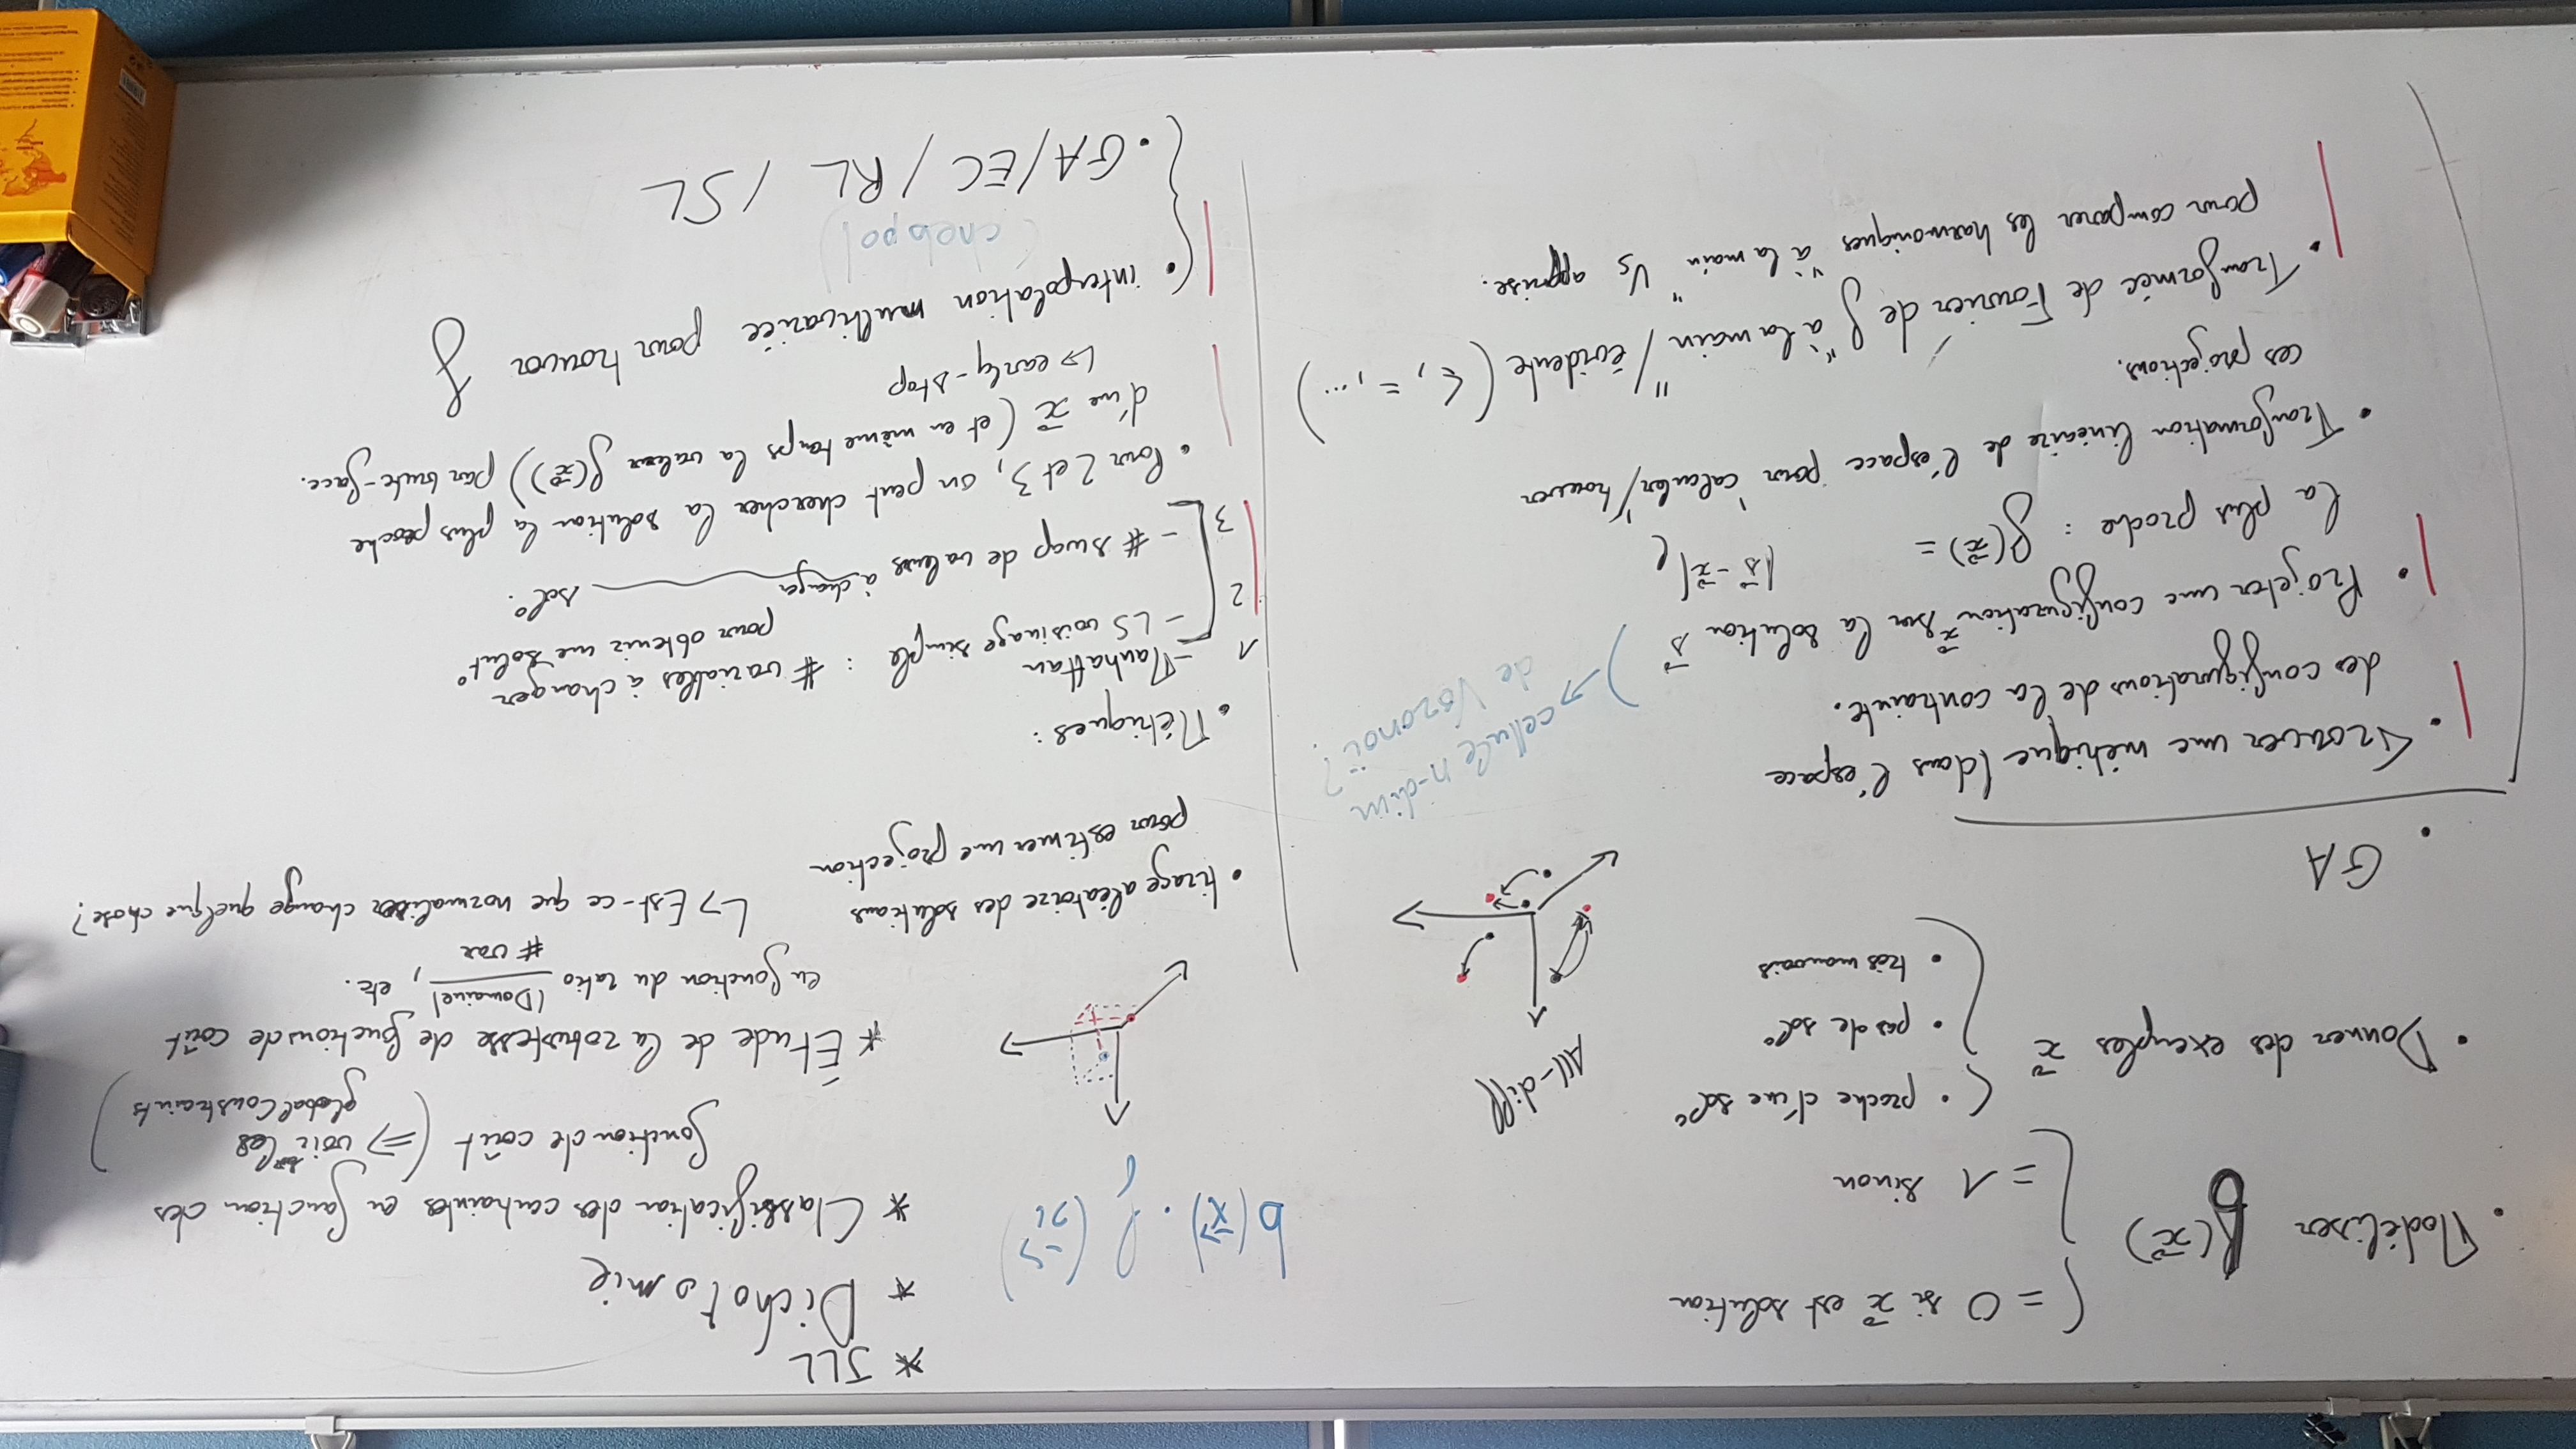
\includegraphics[width=\linewidth,angle=180]{20190529_whiteboard}

\section{Main ideas}
\begin{enumerate}
\item The user must first provide for each constraint type a function $b(\vec{x}) = \left\{
  \begin{array}{rl}
    0 & \text{if } x \text{ is a solution}\\
    1 & y\text{otherwise}
  \end{array} \right.$
$b$ is called ``concept'' in some papers.
\item The goal is to learn $f(\vec x)$ such that the cost function is defined by $b(\vec x) . f(\vec x)$.

\item Find a metric $|.|_l$ in the constraint configuration space. (\danger Space liked to the constraint, since depending one the variables and their domains.)
\item Project the current configuration $\vec{x}$ on the closest solution $\vec{s}$, giving $f(\vec x) = |\vec{s}-\vec{x}|_l$. Need to search for this closest $\vec{s}$ (n-dimensional Voronoï cells?).
\item Fourier transform of the cost function $f'$ of a well-known constraint like all-diff or equality to compare 'hand-designed' harmonics and learned ones.
\item Possible metrics:
  \begin{itemize}
  \item Manhattan: $\sum\limits_i |s[i] - x[i]|$
  \item Hamming: number of variables to change to get a solution (ideal for local search)
  \item Number of swaps of values to get a solution (ideal for permutation constraints).
  \item Manhattan/Hamming mix: Hamming first, then Manhattan as a tie-breaker.
  \end{itemize}
\item Brute-force solution search on small spaces: from a configuration $\vec{x}$, try all possible combinations and test if it is a solution. Early-stop: once we have found a solution, no need to continue the search.
\item The idea is to characterize the cost functions over small instances (few variables/small domains) to make it scale over larger instances.
\item Multivariate  interpolation to find  a scalable formula  for $f$
  (\sout{chebpol} splinter).
\item  Use  of   Genetic  Algorithms/Programming,  other  Evolutionary
  Computation,    Reinforcement    learning,   Supervised    learning?
  $\Rightarrow$ iterative building of cost functions.
\end{enumerate}

\section{Sidekick ideas}
\begin{itemize}
\item[1 bis] The user provides some examples $\vec{x}$ 1. near to be a solution, 2. not a solution but not ridiculous and 3. being a really bad configuration.
\item[3 bis] Could be simplified by a linear transform contracting the constraint configuration space on the manyfold of solutions (so det = 0). Only possible if the manyfold is linear?
\item[5 bis] Random draw of solutions to estimate a projection. Need to know and save solutions somewhere (or to be able to find them quickly).
\item   [6    bis]   See   also   Kantorovich    functional   distance
  from~\cite{StochCP}. See also~\cite{metrics}.
\item [7 bis] Random samplings of the configuration space:
  \begin{enumerate}
  \item Draw a configuration.
  \item Scan all neighbors (with simple '1 variable' neighborhood), or
    sample neighbors (this can be parallelized).
  \item Cost  = numbers of or  mean of neighbors with  a cost strictly
    lesser. Problem: what  are those costs? We are trying  to build it
    actually. Only for iterative processes?
  \end{enumerate}
\item [8 bis] Generate training examples and do reinforcement learning/supervised learning (regression problem)? keeping in mind we look for a function based over the sum of harmonics.
\end{itemize}

\section{Processing data}
\begin{itemize}
\item Normalize samples or apply  a $log_2(x+2)-1$ scaling function to
  diminish potential gaps, in particular  when we have solutions (cost
  = 0).
\item Idea of backward JLL or ``kind of kernel trick'':
  \begin{enumerate}
  \item The user furnishes constraint concepts.
  \item We apply JLL to reduce the space size.
  \item We learn our cost function on this space.
  \item  We apply  some  ``backward  JLL'' to  this  cost function  to
    preserve its properties on the original space.
  \end{enumerate}
\end{itemize}

\section{Formalization}
Define WCSP and CFN such that:
\begin{itemize}
\item  WCSP is  considering soft  constraints, where  a constraint  is
  unsatisfyed iif its associated cost function outputs a value below a
  given threshold $k$ (can be infinite).
\item  CFN  is  considering  hard constraints  only.  Like  constraint
  networks helping solvers to find  solutions by giving a structure of
  the problem,  CFN gives,  in addition of  the constraint  network, a
  structure on  configurations to help  the solver to determine  if an
  unsatisfying configuration is near to be a solution or not.
\item Expressiveness: CFN-sat $<$ WCSP $<$ CFN-opt
\item Reductions/transformation: WCSP $\Rightarrow$ CFN-opt
\end{itemize}

\section{Scaling-related problems}
Several ways to handle scaling.
\begin{enumerate}
\item Learn a function on a small  space and expend it to the original
  space.
\item Draw some samples from the original space
\item Detect and apply symmetries in the original space.
\item Apply JLL to reduce to  original space. maps solutions from this
  space to the compact one, and compute a metric on that compact space
  (eventually learn a function on it).
\end{enumerate}

Problems with those methods so far:
\begin{enumerate}
\item We have no idea how to extend functions with higher cardinality
\item Draw  some samples  does not work  well for  interpolation (10\%
  does not give good results)
\item It is hard to detect AND to correctly apply symmetries.
\item Maybe the solution.
\end{enumerate}

Bonus: what is the point to learn a function if we cannot extend it to
higher spaces?  Computing a  metric on  all points  (or being  able to
compute it on-the-fly quickly) is sufficient.

\subsection{Build solutions incrementally}
If $(x_1,  \ldots, x_{k-1})$  is a  solution, then  try all  values of
$x_k$       with       $(x_k,      x_1,       \ldots,       x_{k-1})$,
$(x_1,         x_k,        \ldots,         x_{k-1})$,        $\ldots$,
$(x_1, \ldots, x_{k-1},  x_k)$. It does not work  with all constraints
(constraint 'sum =  constant' for instance), so with which  ones it is
OK? Being incremental  here means only solutions  on $k-1$ variables
can lead to solutions on $k$ variables.

Classic global constraints in XCSP3-core:
\begin{itemize}
\item regular: \cmark
\item mdd: more a representation than a constraint.
\item allDifferent: \cmark
\item allEqual: \cmark
\item ordered (lessThan extension): \cmark
\item sum: \xmark
\item count: \xmark
\item nValues: \xmark
\item cardinality: \xmark
\item minimum: \xmark
\item maximum: \xmark
\item element: \cmark~for the index version, \xmark~for the membership-only version.
\item channel:  \cmark~but only  adding a variable at  the end
  can lead to solutions.
\item stretch: ???
\item noOverlap: \cmark
\item cumulative: \xmark
\end{itemize}

\section{To explore}
\begin{itemize}
\item Can the Johnson-Lindenstrauss Lemma be useful here?
\item Dichotomy (!?)
\item Constraint classification regarding their cost function.
\item Compute the cost function of the main global constraints.
\item Study the robustness of the cost function regarding the ratio $\frac{|Domain|}{\# vars}$. Does normalization change something?
\item   Compositional  pattern-producing   network  (CPPN~\cite{CPPN})
  instead of the sum of harmonics.
\item For iterative  building (or maybe not):  symmetries detection (=
  free  samples,  see  2.7bis)  should  make  cost  function  building
  faster/easier.
\item Decomposing  complex context  functions given  by the  user into
  some simple functions.
\end{itemize}

\section{Questions / issues}
\begin{itemize}
\item Discrete case of trigonometric functions.
\item How to scale over more variables, like $\text{all-diff}(x, y, z)
  \rightarrow \text{all-diff}(x_1, \ldots, x_n)$
\item How to display an interpoled function on chebpol?
\item Metrics  over the function  space, to  see if two  functions are
  similar or not:
  \begin{itemize}
  \item interpoled function over the  full search space vs. interpoled
    function over samples
  \item interpoled function vs. hand-designed function.
  \end{itemize}
\item Examples of constraints with local minimum? (good to know for cost function iterative building)
\end{itemize}


\bibliographystyle{alpha}
\bibliography{draft}

\end{document}
